\section{Design}
\label{sec:design}

% \begin{figure}[]
%     \centering
%     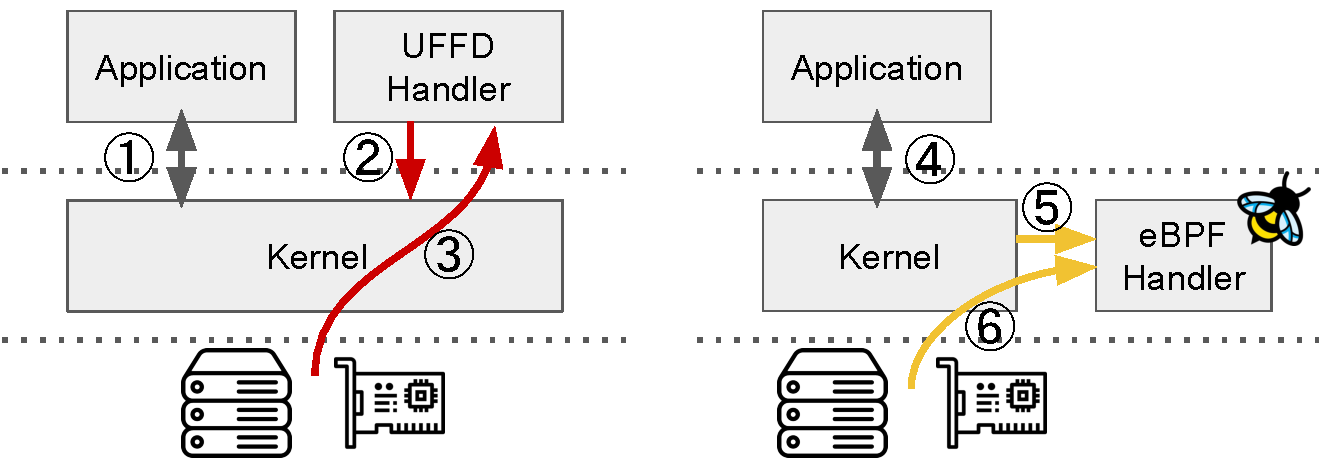
\includegraphics[clip,scale=0.33]{figures/Comparison.pdf}
%     \vspace{-0.5em}
%     \caption{When application triggers page faults (\pgftextcircled{1}, \pgftextcircled{4}), Kernel wakes up uffd handler (\pgftextcircled{2}) or calls eBPF handler (\pgftextcircled{5}). Handler fetches source pages (3, 6), processes them, and returns to kernel. Compared with \pgftextcircled{5} \& \pgftextcircled{6}, \pgftextcircled{2} \& \pgftextcircled{3} incurs overhead with kernel crossing.}
%     \label{fig:motivation-scalability}
%     \vspace{-1.0em}
% \end{figure}

In order to mitigate some of the downsides of \texttt{userfaultfd()}, we propose an \textbf{eBPF-based system} to register custom page fault handlers in-kernel.
%While \texttt{userfaultfd()} has a few different modes of operation, we initially focus on replicating its missing pages functionality.
This system requires two key modifications to the kernel, which we describe in this section.

% Figure xxx is the overall design of our eBPF-powered page fault-handling routine.

\textbf{Per-VMA eBPF programs}. Each eBPF fault-handling program must be associated with a range of the process's address space. The relevant kernel data structure is the \texttt{struct vm\_area\_struct}, which represents a contiguous virtual memory area (VMA). As such, we add support for per-VMA eBPF programs, similar to the kernel's support for per-cgroup eBPF programs~\cite{per-cgroup-bpf}.
After loading and verifying the eBPF program, the application attaches it to a specific address range. The kernel then translates that address range to a VMA (or series of VMAs), and associates the eBPF program with those VMAs.
If the address range starts or ends within a VMA, the kernel will split the VMA, as is done with \texttt{userfaultfd()}.

\textbf{Fault-handling modifications.} We modify the kernel's page fault-handling routine to check if an eBPF program is attached to the relevant VMA. If so, we run the eBPF program, providing metadata about the fault, along with access to a newly allocated page to fill with the desired contents. After the eBPF program executes, we resolve the fault by setting the relevant memory mappings to point to the new page. This removes the need for an additional memory copy, as is done in \texttt{userfaultfd()}, which fills the page in userspace and then copies it into the kernel. We envision this design enabling zero-copy page faults, with data read from the disk or network written directly to the relevant page.

For simple fault-handling routines, the aforementioned kernel changes should be sufficient. However, for more complex applications such as VM migration which require reading data from the network or disk, we envision adding eBPF helpers to support such operations, along with building on the existing support for sleepable eBPF programs~\cite{sleepable-bpf}.

We believe that this implementation removes the need for an additional fault-handling thread and reduces unnecessary kernel crossings or data copying. While eBPF may somewhat limit the flexibility of the custom fault handlers, we believe that eBPF is mature enough to handle interesting and complex use cases. Additionally, the eBPF verifier could be used to limit the operations used in the handling routine, such as sleeping indefinitely, potentially addressing the security concerns that plague \texttt{userfaultfd()}.
